% !TeX root = ../Thesis.tex

%************************************************
\chapter{Implementation}\label{ch:implementation}
%************************************************
\glsresetall % Resets all acronyms to not used

In this chapter, we want to discuss the details of our implementation of text-based steganography on Android. First we will give a high-level overview of the app in \cref{sec:overviewOfTheApp}. Then \cref{sec:jni} will show an example of how Java/Kotlin and C++ code can interact using the \gls{JNI}. \cref{sec:tokenGenerationWithLlamaCpp} will introduce all necessary abstractions to understand token generation with llama.cpp. \cref{sec:algorithms} will explain the algorithms we used for steganography. So far, this is what was needed to port the functionality of Stegasuras~\cite{zieglerNeuralLinguisticSteganography2019} to Android.

We expand this functionality already in \cref{sec:algorithms} by implementing another compression algorithm. Then we will show how to improve cover text quality in \cref{sec:finishingTheLastSentence,sec:creatingAConversationBetweenCoverTexts,sec:emojis}: First we will show how to handle the last sentence, then how to create a conversation, and lastly how to generate emojis.

\section{Overview of the app}
\label{sec:overviewOfTheApp}
In this section, we will give a high-level overview of the app. We walk through every screen of the \gls{UI} and explain what functionality is offered and how to use it.

\subsection{Home screen}
\label{sec:homeScreen}
\cref{fig:homeScreen} shows the home screen of our app. The \gls{UI} is based on the Stegasuras demo~\cite{zieglerStegasuras2025}: We have two text input fields, a mode selector for encode/decode, a switch to toggle conversation on/off, and a start button. Furthermore, we have icons in the top corners for navigation to the other screens (see \cref{sec:conversationScreen,sec:settingsScreen}).

\begin{figure}
	\begin{wide}
		\captionsetup{width=\linewidth}
		\begin{subfigure}{0.45\linewidth}
			\centering
			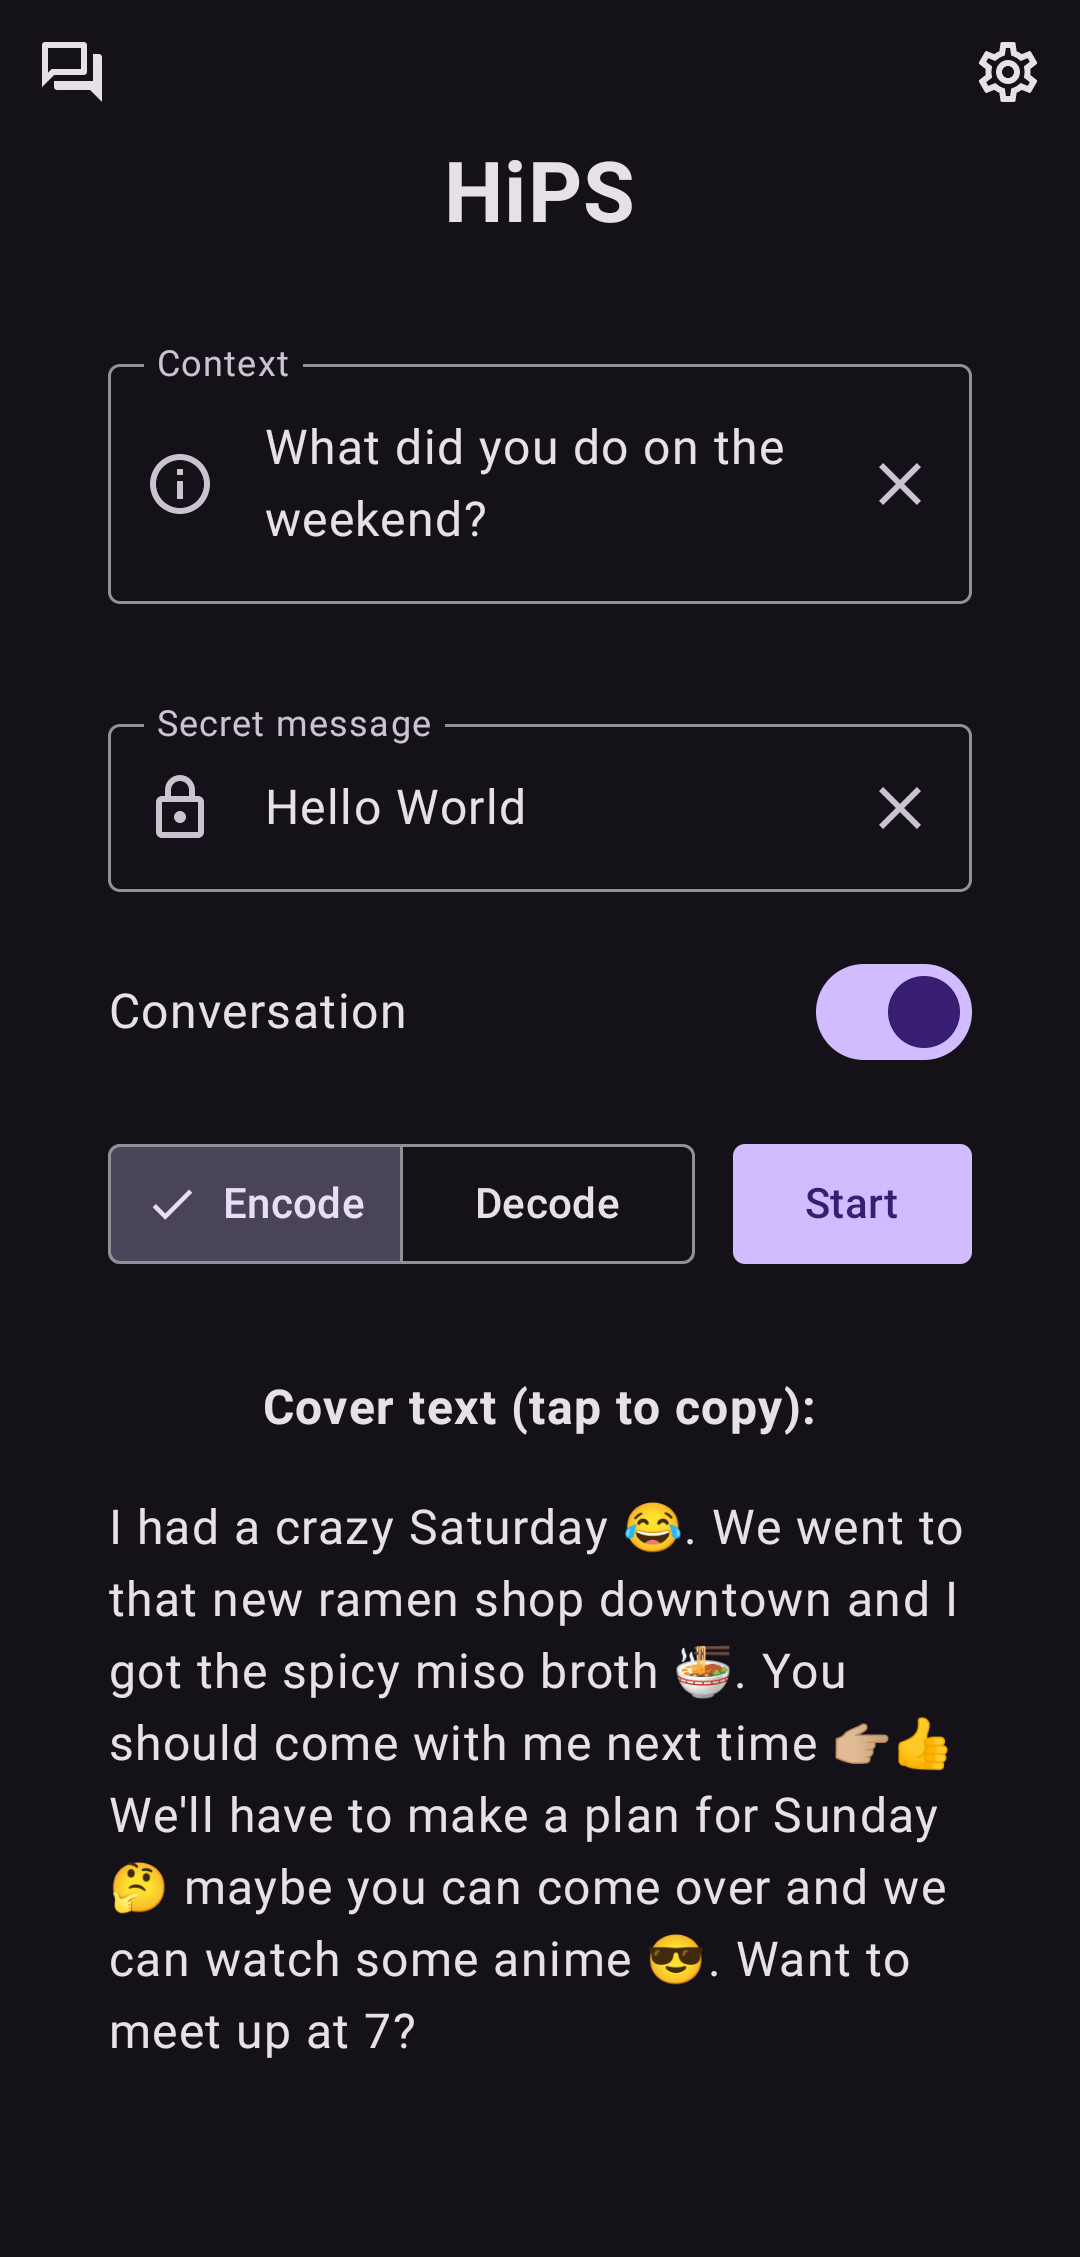
\includegraphics[width=\linewidth]{hips_home_screen_a.png}
			\caption{Encoding of a secret message.}
			\label{fig:homeScreenA}
		\end{subfigure}
        \hfill
		\begin{subfigure}{0.45\linewidth}
			\centering
			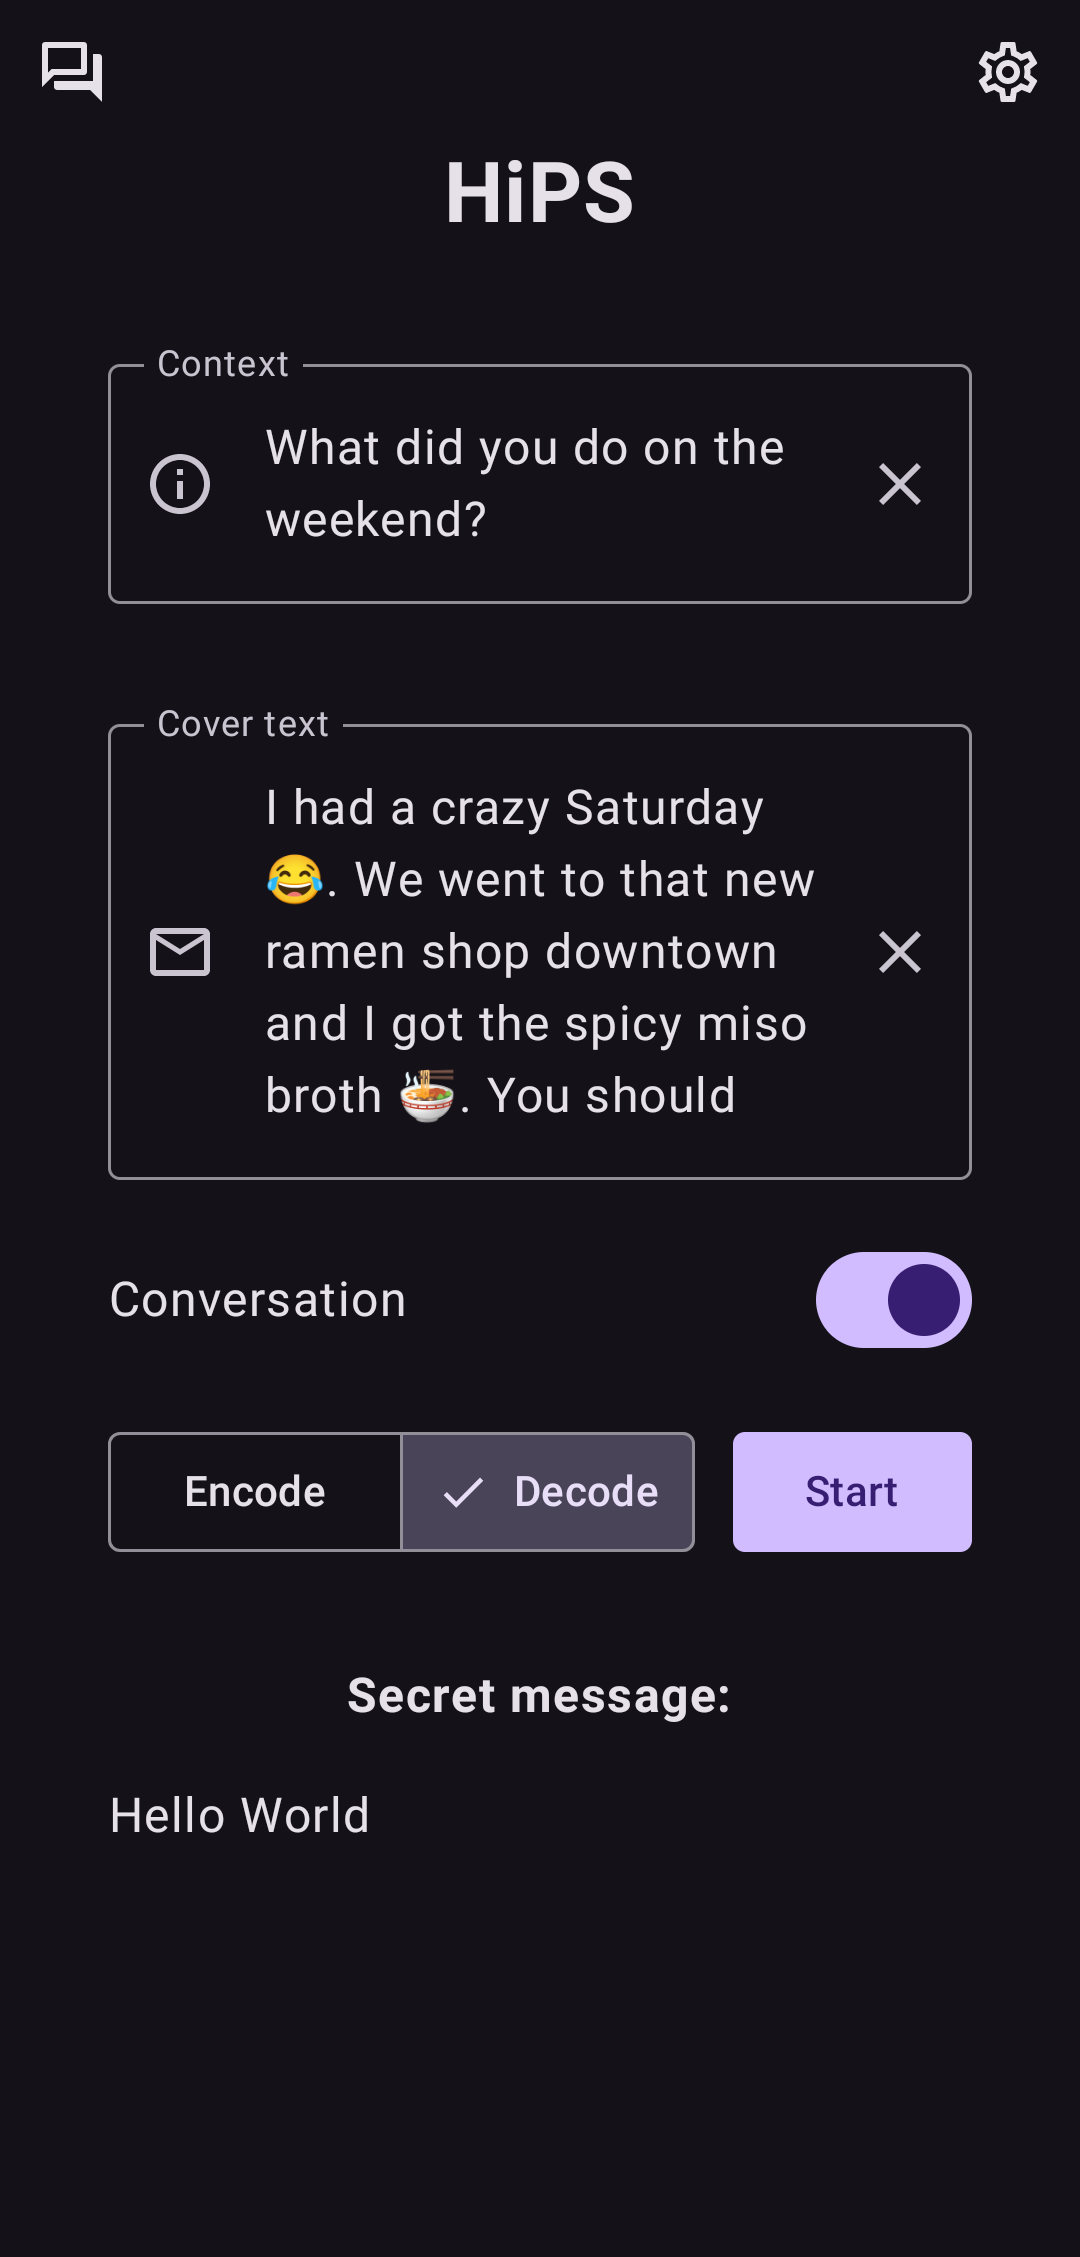
\includegraphics[width=\linewidth]{hips_home_screen_b.png}
			\caption{Decoding of a cover text.}
			\label{fig:homeScreenB}
		\end{subfigure}
		\caption[HiPS: Home screen]{Standalone functionality of HiPS on the home screen.}
		\label{fig:homeScreen}
	\end{wide}
\end{figure}

In encode mode, the text input fields are for the context to generate a cover text from, and for the secret message to be encoded in the cover text. After pressing the start button, the cover text will be generated and displayed at the bottom. Tapping it copies it to the clipboard. In decode mode, the text input fields are for the context the cover text. After pressing the start button, the secret message will be display at the bottom.

The functionality of Stegasuras is replicated by toggling the conversation switch off. The cover text is then generated by \textit{completing} the context. This opens up adjacent use cases, e.g. using a press statement to transfer information out of an organization.

When the conversation switch is toggled on, the functionality of Stegasuras is extended. The cover text is then generated by \textit{replying} to the context, i.e. the context is assumed to be a chat message. This uses the settings configurable on the settings screen (see \cref{sec:settingsScreen}). This standalone functionality helps users protect their privacy with existing instant messengers by simply copy-pasting messages.

\subsection{Conversation screen}
\label{sec:conversationScreen}
\cref{fig:conversationScreen} shows the conversation screen. This is a demo of how our steganography could be integrated into an instant messenger.

\begin{figure}
	\begin{wide}
		\captionsetup{width=\linewidth}
		\begin{subfigure}{0.45\linewidth}
			\centering
			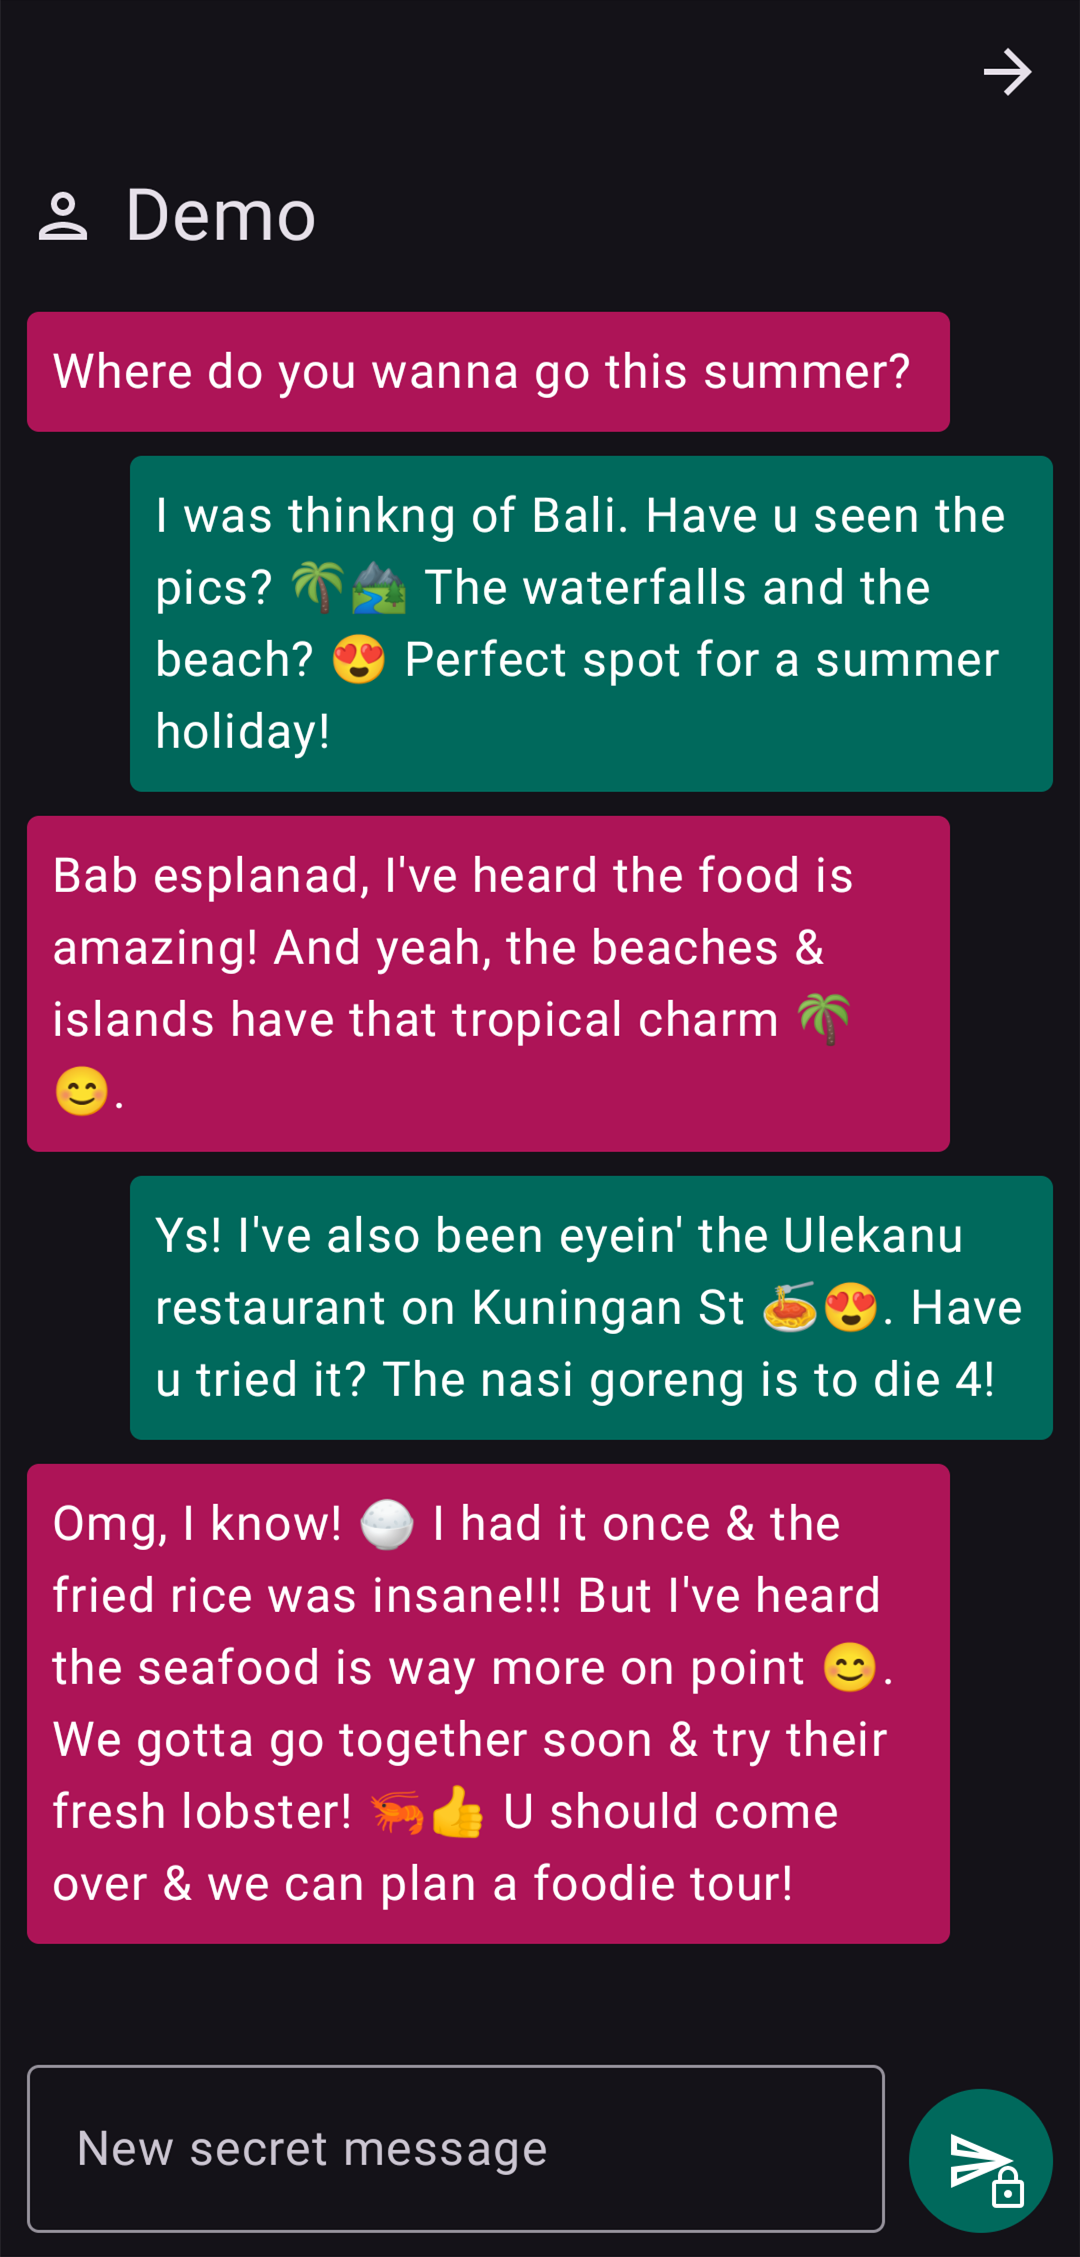
\includegraphics[width=\linewidth]{hips_conversation_screen_a.png}
			\caption{A conversation of cover texts.}
			\label{fig:conversationScreenA}
		\end{subfigure}
        \hfill
		\begin{subfigure}{0.45\linewidth}
			\centering
			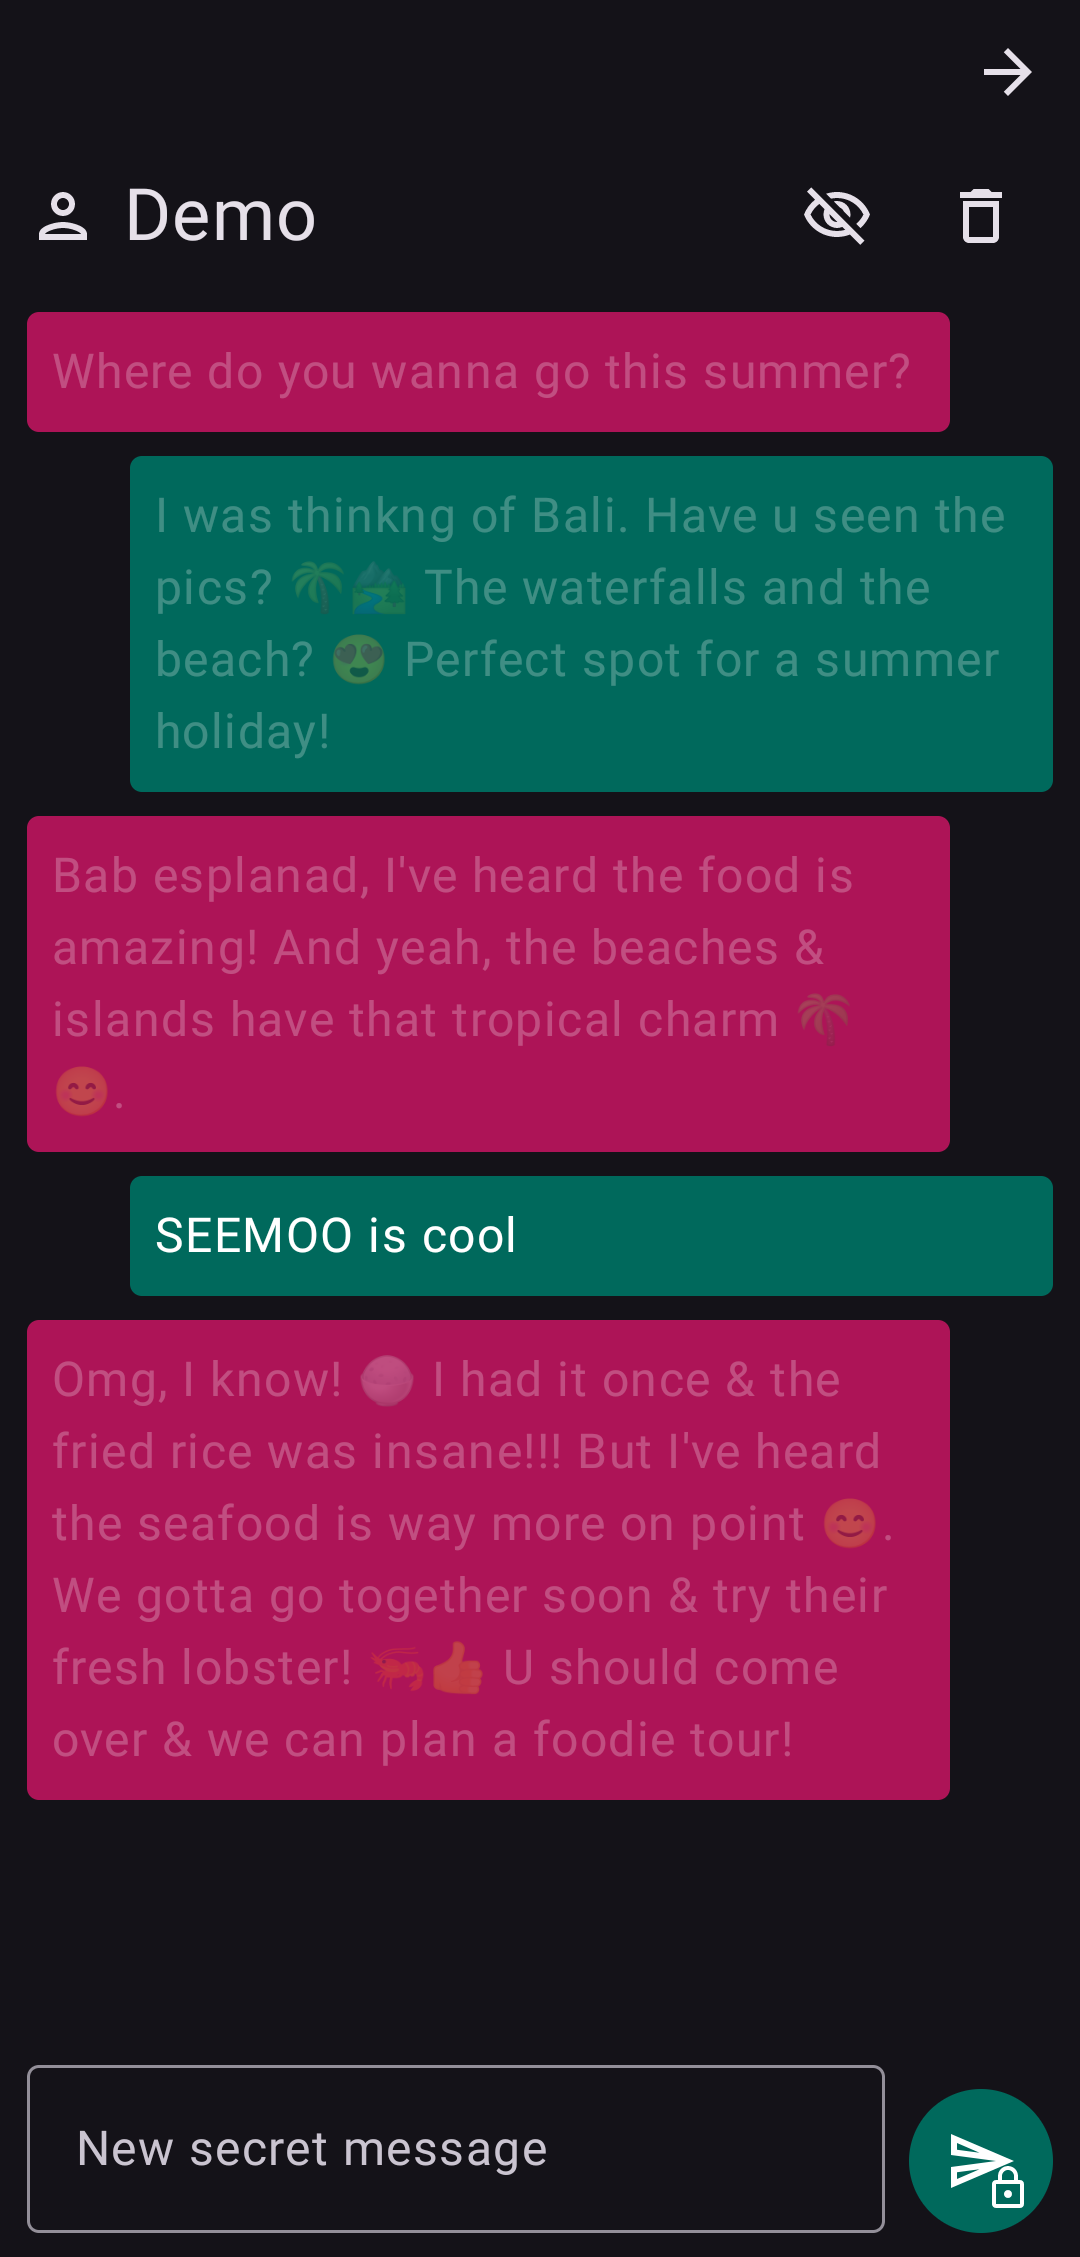
\includegraphics[width=\linewidth]{hips_conversation_screen_b.png}
			\caption{Showing a secret message.}
			\label{fig:conversationScreenB}
		\end{subfigure}
		\caption[HiPS: Conversation screen]{Steganography on the conversation screen.}
		\label{fig:conversationScreen}
	\end{wide}
\end{figure}

This screen displays a list of messages, a text input field and a send button. The messages are arranged as a chat conversation between two people and coloured correspondingly. The text input field allows the user to type in a new message, which then can be sent into the chat by pressing the send button. As this is a demo, they are not sent over the internet, but only stored locally. Effectively, the users chat with themselves by constantly switching roles. At the top, we have placeholders for name and profile picture of the chat partner, and a back button to navigate back to the home screen.

The send button can be long-pressed to toggle steganography on/off. The current mode is indicated by a lock being shown or hidden inside it. If steganography is toggled on, the message in the text input field is assumed to be a secret message and will be encoded into a cover text. The cover text is then sent into the conversation. Again, this can be configured on the settings screen (see \cref{sec:settingsScreen}): The system prompt and a number of prior messages are used as context to generate the cover text from. This corresponds to the conversation switch on the home screen being toggled on (see \cref{sec:homeScreen}). If steganography is toggled off, the message in the text input field is assumed to be a plain text message and will be sent as is. This allows for arbitrary plain text messages in-between cover texts.

When the text input field is blank, the send button can be short-pressed to switch roles. The current role is indicated by the send button being the same colour as the corresponding messages. This allows for sending multiple consecutive messages from the same role, i.e. roles to not be strictly alternating. The role also switches automatically after sending a message. Messages in the chat can also be long-pressed, which highlights them as being selected. Short-pressing unselects them again. If at least one message is selected, two new buttons will be displayed at the top: Decode and delete.

The decode button can only be pressed if exactly one message is currently selected. Otherwise, a toast is displayed to guide the user. This is to avoid running multiple instances of the \gls{LLM} simultaneously. Otherwise, the app process could be terminated by the Android operating system for excessive resource usage. When the decode button is pressed, it tries to decode the selected message. If decoding was successful (i.e. if the selected message was a cover text and not a plain text), the secret message will be displayed in place of the cover text. The symbol of the decode button changes to indicate that a secret message is visible. By pressing it again, the secret message and the two buttons are hidden again.

The delete button can only be pressed if the selected messages are at the end of the conversation. Otherwise, a toast is displayed again. This is to avoid corrupting the context for decoding a message by deleting messages prior to it. When the delete button is pressed, the selected messages will be deleted and the two buttons will be hidden again.

\subsection{Settings screen}
\label{sec:settingsScreen}
\cref{fig:settingsScreen} shows the settings screen. This is where the \gls{LLM} is managed and where all parameters of our algorithms can be modified. Upon installation of our app, the user needs to download the \gls{LLM} by pressing the download button at the top of this screen. Then the \gls{LLM} can be loaded into or unloaded from memory by pressing the start/stop button below the download button. Pressing this button is only necessary after downloading the \gls{LLM} when using our app for the first time. Afterwards, the \gls{LLM} is automatically loaded on startup.

\begin{figure}
	\begin{wide}
		\captionsetup{width=\linewidth}
		\begin{subfigure}{0.3\linewidth}
			\centering
			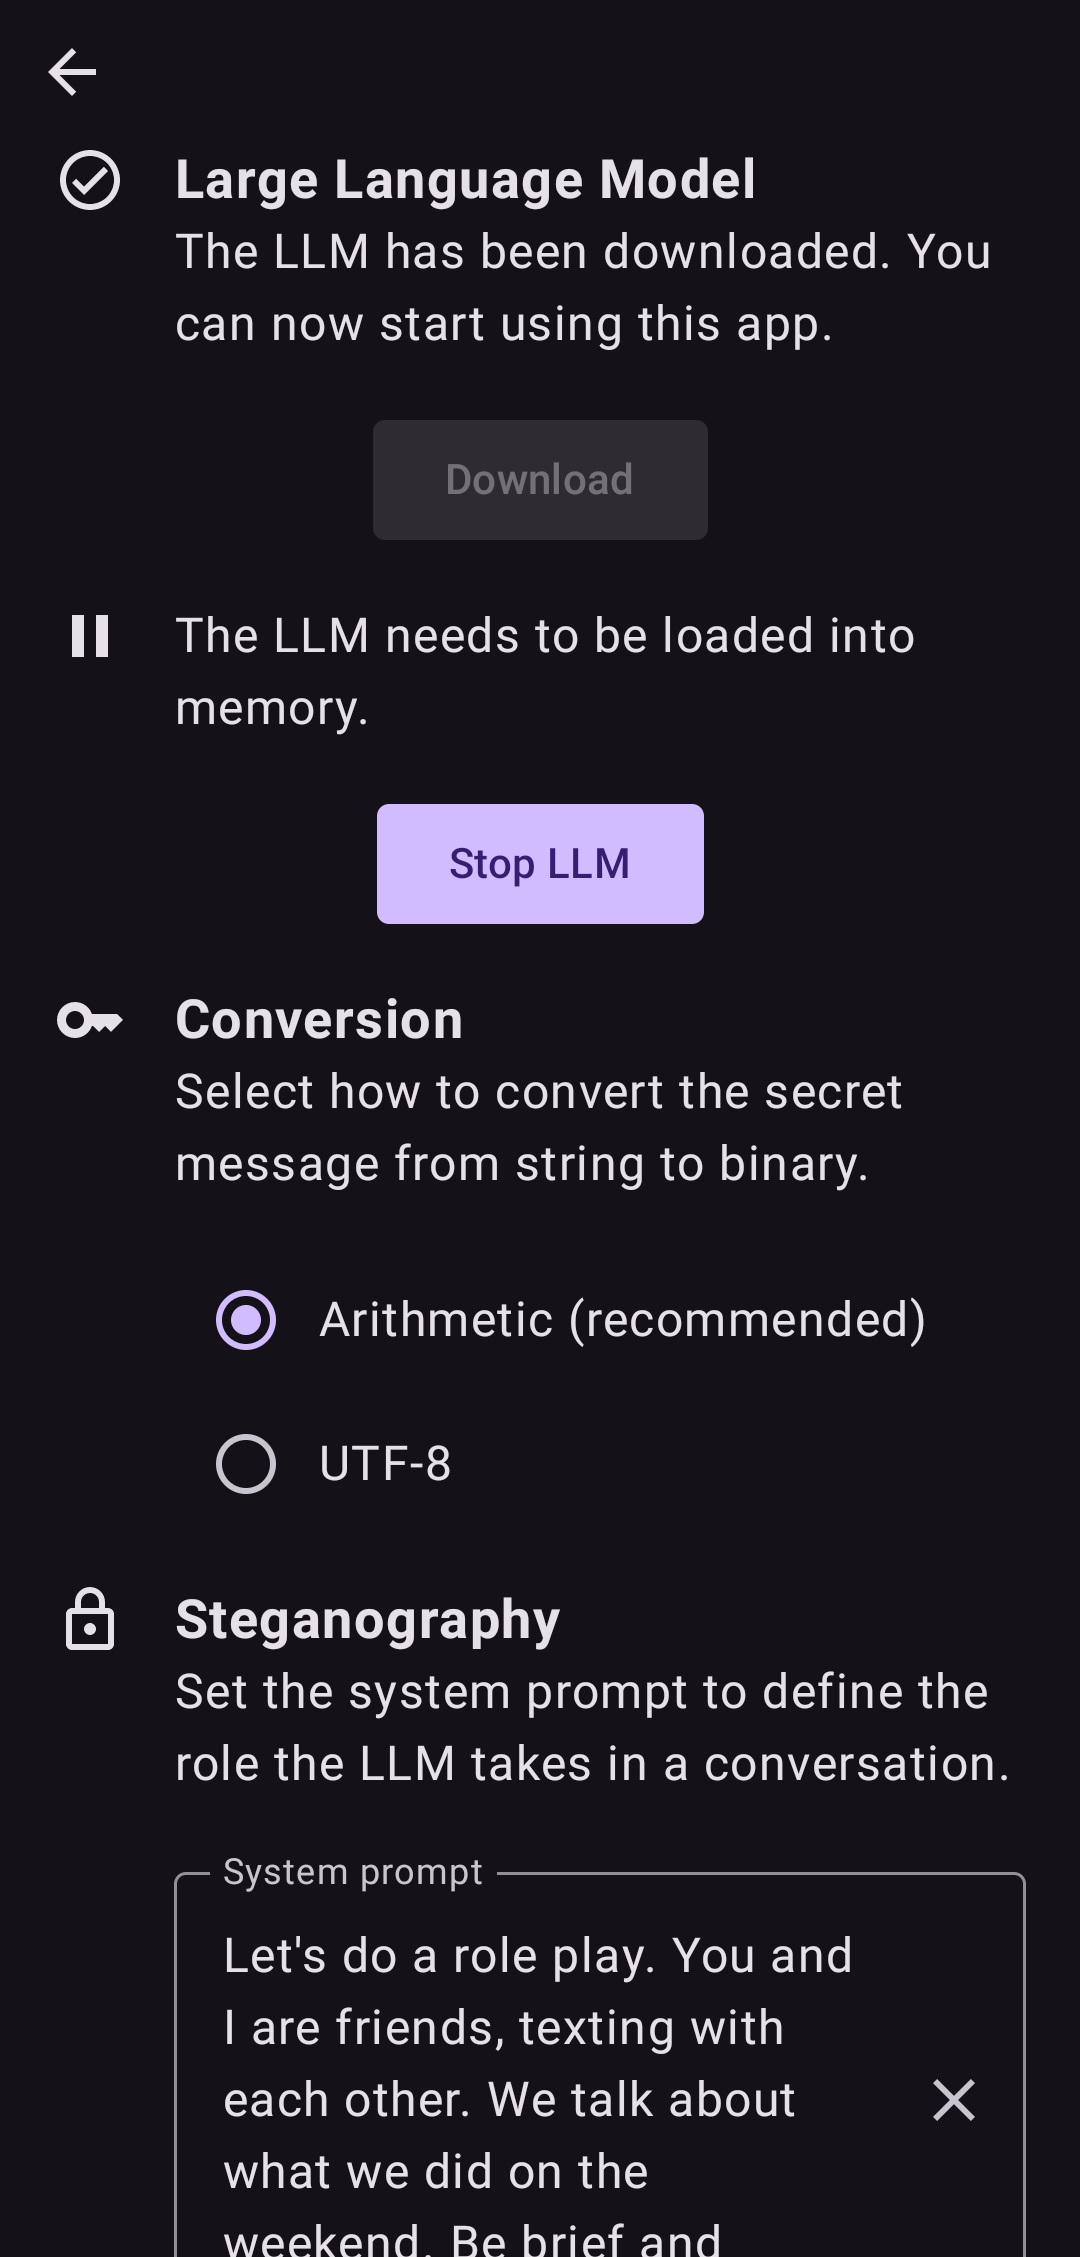
\includegraphics[width=\linewidth]{hips_settings_screen_a.png}
			\caption{Download button, start button and binary conversion mode.}
			\label{fig:settingsScreenA}
		\end{subfigure}
        \hfill
        \begin{subfigure}{0.3\linewidth}
			\centering
			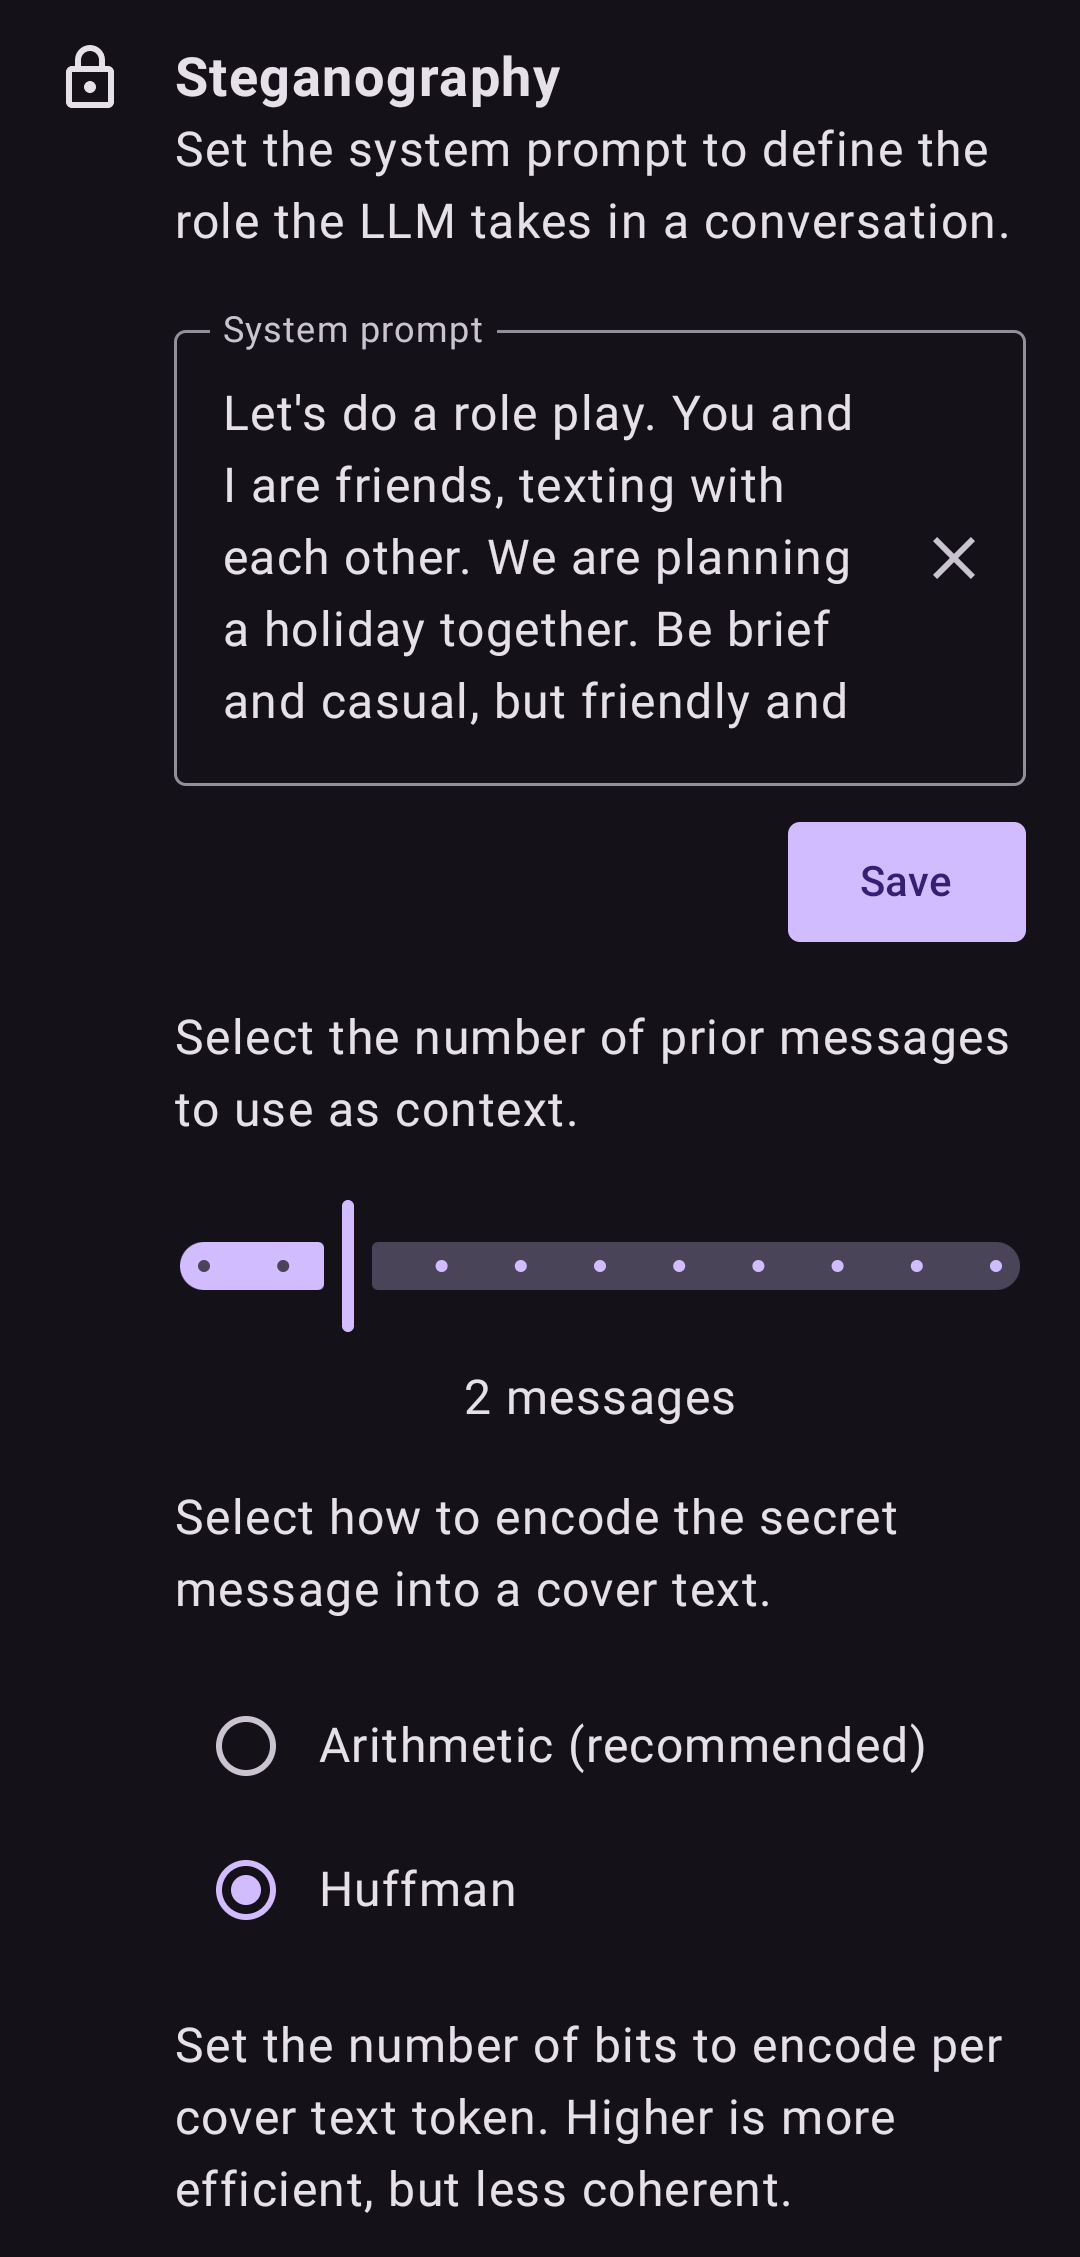
\includegraphics[width=\linewidth]{hips_settings_screen_b.png}
			\caption{System prompt, context length and steganography mode.}
			\label{fig:settingsScreenB}
		\end{subfigure}
        \hfill
        \begin{subfigure}{0.3\linewidth}
			\centering
			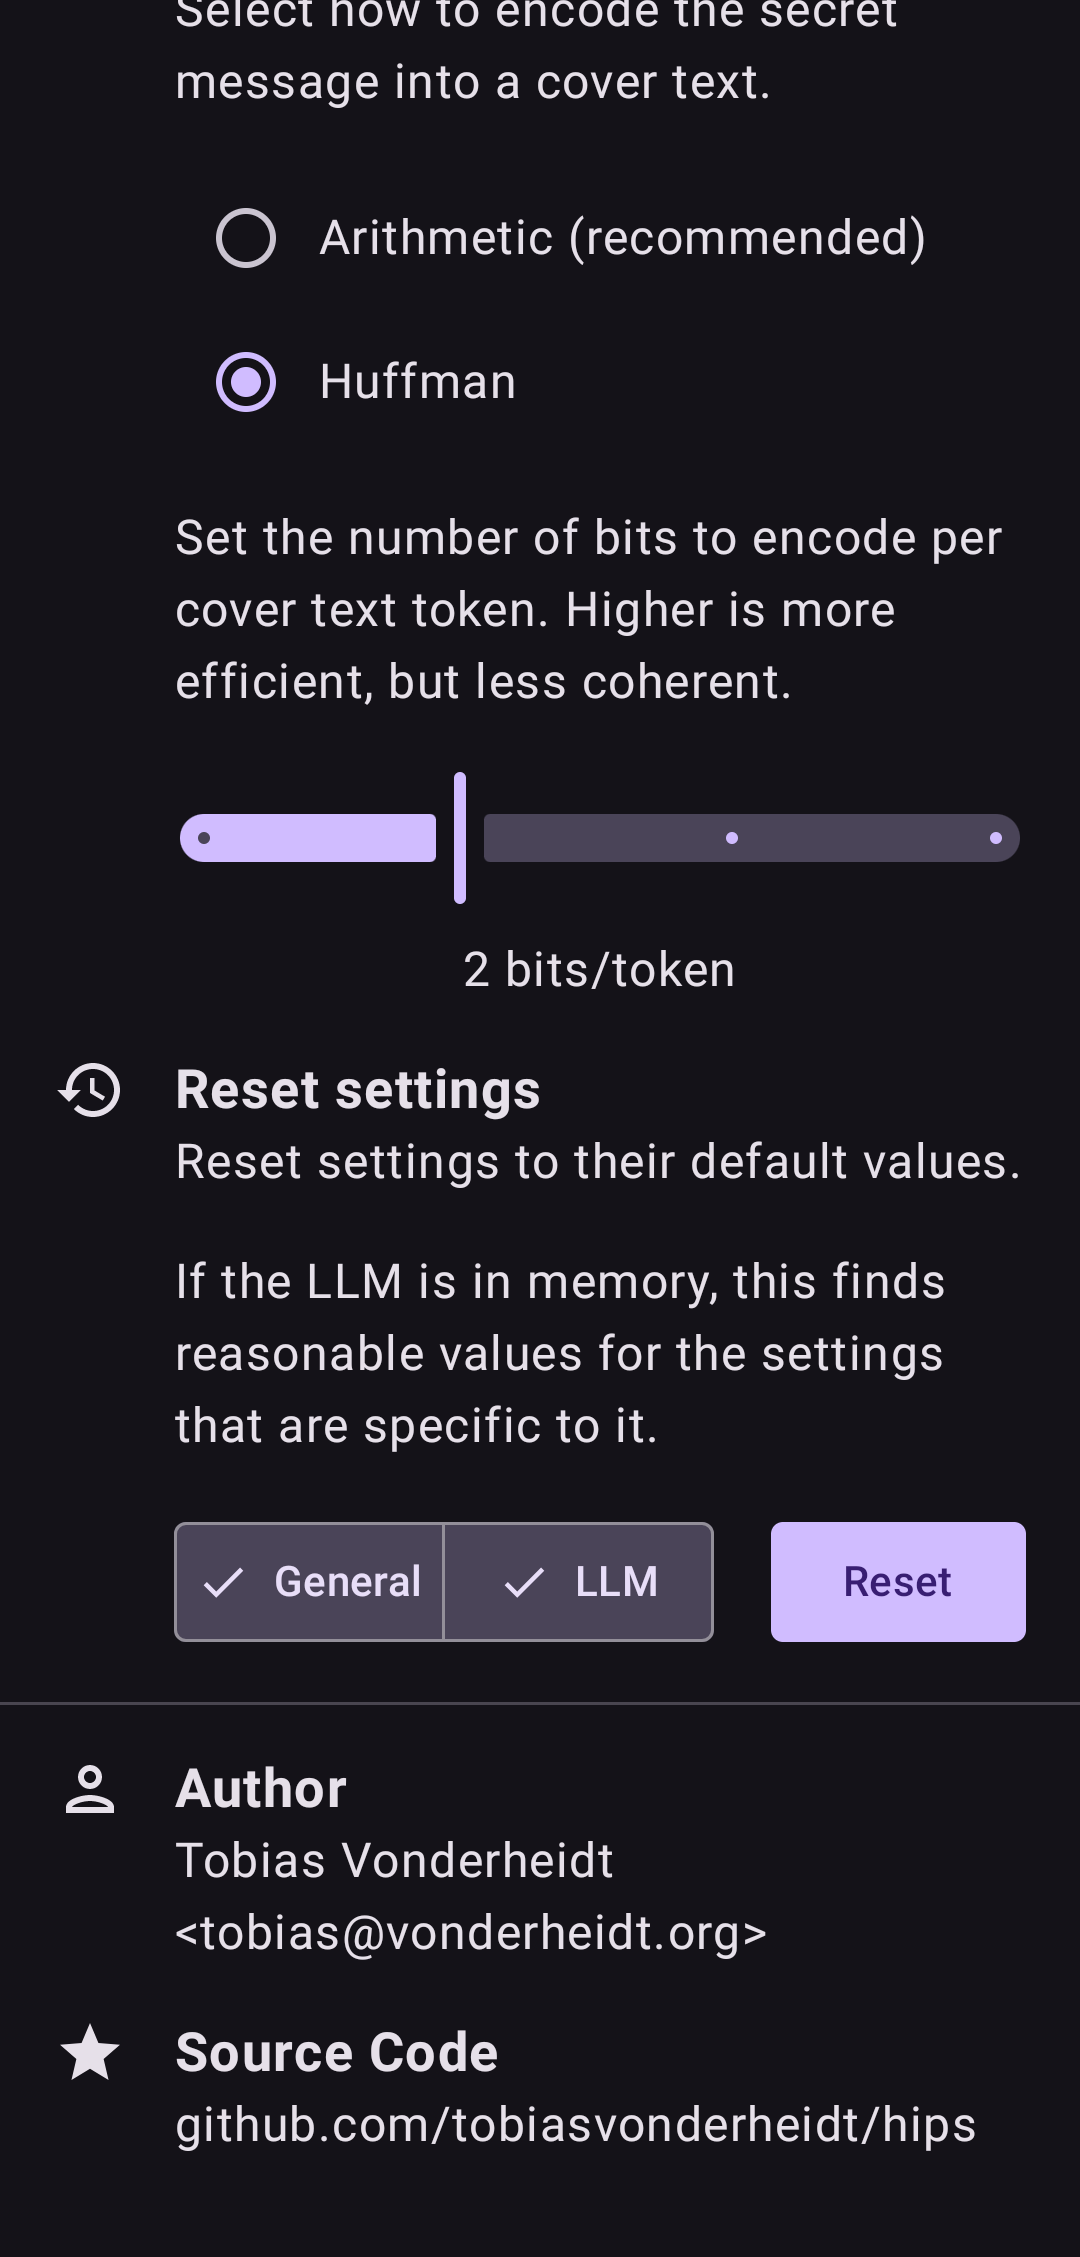
\includegraphics[width=\linewidth]{hips_settings_screen_c.png}
			\caption{Algorithm-specific settings for Huffman coding and reset options.}
			\label{fig:settingsScreenC}
		\end{subfigure}
		\caption[HiPS: Conversation screen]{The settings screen.}
		\label{fig:settingsScreen}
	\end{wide}
\end{figure}

Below these buttons, there are various selectors, sliders and input fields for the parameters of our algorithms. They are arranged in the order of corresponding steps during the encoding process. First there is a selector for the conversion mode, i.e. for how to convert the secret message from string to binary. It offers \lstinline|Arithmetic (recommended)|, \lstinline|Huffman| and \lstinline|UTF-8| as options. \lstinline|UTF-8| serves as a baseline as it doesn't compress the secret message, while \lstinline|Arithmetic| compresses it using the \gls{LLM} and \lstinline|Huffman| compresses it without using the \gls{LLM}. This will be explained in detail in \cref{sec:binaryConversionAndCompression}.

This is followed by a text input field for a system prompt. This is a natural language command that can be passed to the \gls{LLM} to influence its behaviour. This is relevant for the conversation screen, and for the home screen if the conversation switch there is toggled on. A more detailed explanation for how the system prompt is used will be given in \cref{sec:creatingAConversationBetweenCoverTexts}.

Afterwards, there is a slider to select a number of messages between 0 and 10. This is the number of prior messages to be used as context on the conversation screen. It is not relevant for the home screen, as context length is always fixed to 1 message there. While values 1 to 10 be used as is, 0 is interpreted as \lstinline|All messages|. This means, all prior messages will be used as context to generate the next cover text from. It is recommended to set this to a value in the 1-10 range to limit resource usage when a conversation contains many messages.

Furthermore, we have a selector for the steganography algorithm. It offers \lstinline|Arithmetic (recommended)| and \lstinline|Huffman| as options. Depending on the selected algorithm, its specific parameters can be set below this selector (see \cref{sec:steganographyEncodingDecoding} for details).

When \lstinline|Arithmetic| is selected, there are sliders for the \lstinline|temperature|, \lstinline|topK| and \lstinline|precision| parameters. The \lstinline|temperature| slider ranges from 0.0 to 2.0 in steps of 0.1, but can't be 0.0 as we will need to divide by the \lstinline|temperature| value. The \lstinline|topK| slider ranges from 0 to 100\% of the vocabulary size of the \gls{LLM}. The \lstinline|precision| slider ranges from 0 to 32 bits. Both \lstinline|topK| and \lstinline|precision| are only visible when the \gls{LLM} is in memory, as the vocabulary size for \lstinline|topK| is specific to each \gls{LLM} and the recommended value for \lstinline|precision| depends on it.

When \lstinline|Huffman| is selected, there is a slider for the \lstinline|bitsPerToken| parameter. It determines the height of the Huffman tree and therefore the bits encoded in every cover text token. The slider ranges from 0 to 4.

Lastly, there is a button to reset all settings to their default values. It comes with a selector for whether to reset either only general settings, only settings that are specific to the \gls{LLM} (i.e. \lstinline|topK| and \lstinline|precision|), or both. When the \gls{LLM} is in memory, settings specific to it will be reset to sensible defaults. Otherwise, they are reset to 0.

\section{Java Native Interface}
\label{sec:jni}
As discussed in \cref{sec:llamaCpp}, we chose llama.cpp as the framework to run our \glspl{LLM} with. Since this is a C++ library, we will need to integrate C++ code into our Kotlin-based Android app. This is facilitated by using the \gls{JNI}. It allows us to declare Kotlin functions as \lstinline|external|, signalling that their implementation is done in C++ rather than Kotlin. Arguments and return values can then be passed back and forth.

Listings~\ref{lst:jniKotlin} and~\ref{lst:jniCpp} show examples for this: On the Kotlin side, the \gls{LLM} instance is represented by the \lstinline|LlamaCpp| class. More specifically, \lstinline|LlamaCpp| is an object. This is the Kotlin syntax for a singleton class. Multiple instances of the \gls{LLM} are avoided this way. On the C++ side, there are only the corresponding function implementations. The C++ functions are mostly wrappers for llama.cpp function calls. Inputs and outputs need to be converted between Kotlin and C++ data types, but most logic is implemented on the Kotlin side. While this design decision may introduce performance drawbacks (see \cref{ch:evaluation}), it makes maintenance significantly easier.

% Add some space on top of listing to match bottom
\vspace{0.25cm}

\begin{lstlisting}[caption={[JNI: Kotlin side]{Example for the Kotlin side of the \gls{JNI}: State management for the \gls{LLM} using a function declared \lstinline|external| at the end.}}, label={lst:jniKotlin}]
object LlamaCpp {
    @Volatile
    private var model = 0L

    fun isInMemory(): Boolean {
        return model != 0L
    }

    fun startInstance() {
        if (isInMemory()) {
            return
        }

        synchronized(lock = this) {
            if (!isInMemory()) {
                model = loadModel()
            }
        }
    }

    private external fun loadModel(path: String): Long
}
\end{lstlisting}

% Move following paragraphs here to avoid page break in next listing
On the Kotlin side, the \gls{LLM} is loaded into memory by calling the \lstinline|loadModel| function with the path to a \lstinline|.gguf| file as a string argument. This function is declared \lstinline|external|, so its implementation is in C++. On the C++ side, the Kotlin string is converted to a C++ string via the \gls{JNI}. In turn, the \lstinline|llama_model_load_from_file| function of llama.cpp is called, which takes the file path as C++ string and some default parameters as arguments. This returns the memory address of the \gls{LLM} as a pointer. Pointers only exist in C++, but can be cast to Kotlin long numbers as both are 64 bits in size. Therefore, \lstinline|loadModel| returns a Kotlin long number. This is stored in the attribute \lstinline|model| of the \lstinline|LlamaCpp| object, so the state of the \gls{LLM} can be managed: If \lstinline|model| is 0, the \gls{LLM} is not in memory. Otherwise it is and can be referenced via this attribute.

The \lstinline|startInstance| function loads of the \gls{LLM} in a thread-safe manner by implementing a double-checked locking mechanism~\cite{ishizakiTransformingJavaPrograms2014}. This is commonly used with singleton classes in Java, and by extension, Kotlin. Unloading the \gls{LLM} mirrors this.

% Add some space on top of listing to match bottom
\vspace{0.25cm}

\begin{lstlisting}[caption={[JNI: C++ side]{Example for the C++ side of the \gls{JNI}: Implementation of the function declared \lstinline|external| in Listing~\ref{lst:jniKotlin}.}}, label={lst:jniCpp}]
extern "C" JNIEXPORT jlong JNICALL Java_org_vonderheidt_hips_utils_LlamaCpp_loadModel(JNIEnv* env, jobject /* thiz */, jstring jPath) {
    jboolean isCopy = true;

    const char* cppPath = env -> GetStringUTFChars(jPath, &isCopy);

    llama_model_params params = llama_model_default_params();

    llama_model* cppModel = llama_model_load_from_file(cppPath, params);

    env -> ReleaseStringUTFChars(jPath, cppPath);

    auto jModel = reinterpret_cast<jlong>(cppModel);

    return jModel;
}
\end{lstlisting}

\section{Token generation with llama.cpp}
\label{sec:tokenGenerationWithLlamaCpp}
In this section, we explain how token generation works with llama.cpp, i.e. how the \gls{LLM} generates text. We focus on the abstractions needed to work with llama.cpp, omitting any more general concepts. Most of this explanation is based on a great blog post by Omri Mallis~\cite{mallisUnderstandingHowLLM2023} and the examples given in the llama.cpp GitHub repository~\cite{gerganovGgerganovLlamacpp2024}. \cref{fig:llamaCppTokenGeneration} shows the high-level flow we need to understand.

\begin{figure}
    \begin{wide}
        \captionsetup{width=\linewidth}
        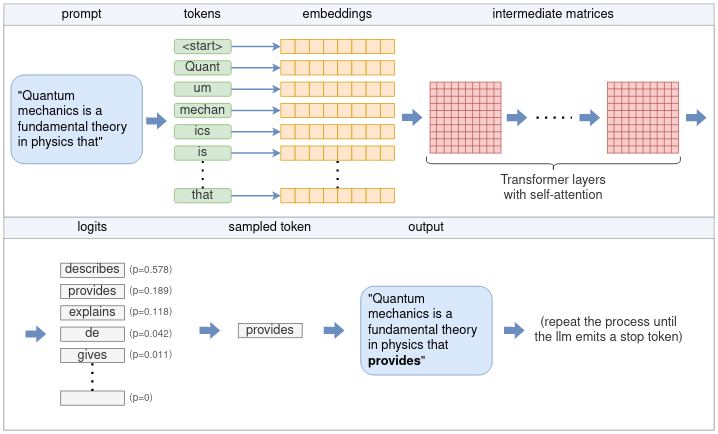
\includegraphics[width=\linewidth]{llama_cpp_high_level_flow.png}
        \caption[llama.cpp: Token generation]{High-level flow of token generation in llama.cpp~\cite{mallisUnderstandingHowLLM2023}.}
        \label{fig:llamaCppTokenGeneration}
    \end{wide}
\end{figure}

Fundamentally, \glspl{LLM} iteratively complete any text they are given as input~\cite{mallisUnderstandingHowLLM2023}. We call this input a prompt. The generated completion is returned as output. We call this output the response. In \cref{fig:llamaCppTokenGeneration}, the prompt is "Quantum mechanics is a fundamental theory of physics that" and the response (after one iteration) is "provides"~\cite{mallisUnderstandingHowLLM2023}.

First, we need to understand an important distinction: The \gls{LLM} and its state. In the llama.cpp source code, the \gls{LLM} is called \lstinline|model|. Its state is called \lstinline|ctx| (short for context)~\cite{gerganovGgerganovLlamacpp2024}. The \lstinline|model| itself is stateless. This can be demonstrated by its idempotence: Consider one instance of a \lstinline|model| with an empty \lstinline|ctx|. When it is given a prompt, it will return a response. Reset the \lstinline|ctx| so it is empty again. If you give it the same prompt now, you will receive the same response again. Resetting the \lstinline|object| is important in our implementation to ensure reproducible results.

A \lstinline|ctx| takes the memory address of a \lstinline|model| as argument when being created~\cite{gerganovGgerganovLlamacpp2024}. Thereby, it is attached to the \lstinline|model| instance. Token generation only needs to access the \lstinline|ctx|. Resetting the \lstinline|ctx| works by unloading it from memory and loading a new \lstinline|ctx| attached to the same \lstinline|model| instance into memory. The implementation is analogous to loading and unloading the \gls{LLM} as shown in \cref{sec:jni}. However, the following paragraphs will only refer to the \gls{LLM} for readability, abstracting the \lstinline|ctx| away.

The \gls{LLM} starts processing the prompt by tokenizing it. This means that the prompt is not just split into words, but dismantled further into sub-word units called tokens~\cite{mallisUnderstandingHowLLM2023}. In \cref{fig:llamaCppTokenGeneration}, for example the word "Quantum" is composed of the tokens "Quant" and "um". A token can be represented as a string, which is depicted in~\cref{fig:llamaCppTokenGeneration}, or as an integer, which is then called the token ID~\cite{mallisUnderstandingHowLLM2023}. After tokenization, the \gls{LLM} first works with the token IDs before converting the tokens further into other representations (see below).

A common tokenization algorithm is \gls{BPE}~\cite{sennrichNeuralMachineTranslation2016}. Popular tokenizers using \gls{BPE} include Google's SentencePiece~\cite{googleGoogleSentencepiece2024}, which is used in Stegasuras~\cite{zieglerHarvardnlpNeuralSteganography2025,zieglerStegasuras2025}, and OpenAI's TikToken~\cite{openaiOpenaiTiktoken2025}, which is used in our \gls{LLM} of choice, Llama 3.2 1B~\cite{metaMetallamaLlamamodels2025}.

In llama.cpp, the tokens to be processed are stored in a separate data structure called a \lstinline|batch|. During the first iteration, the batch contains all tokens of the prompt. During subsequent iterations, the batch only contains the last sampled token (see below for a definition of sampling)~\cite{gerganovGgerganovLlamacpp2024}.

To complete the prompt, the \gls{LLM} needs to predict which tokens are likely to come next. To be comparable, the tokens need to be converted into a more structured representation. Each token in the prompt is converted into a vector, called an embedding~\cite{mallisUnderstandingHowLLM2023}. These vectors can be stacked to form the embedding matrix~\cite{mallisUnderstandingHowLLM2023}. \cref{fig:llamaCppEmbedding} shows the embedding matrix in detail. Its dimensions are \lstinline|n_tokens| $\times$ \lstinline|n_embd|. \lstinline|n_tokens| is the number of tokens in the prompt. \lstinline|n_embd| is the dimension of the vectors representing the tokens, which is specific to each \gls{LLM}~\cite{mallisUnderstandingHowLLM2023}.

\begin{figure}
    \begin{wide}
        \centering
        \captionsetup{width=\linewidth}
        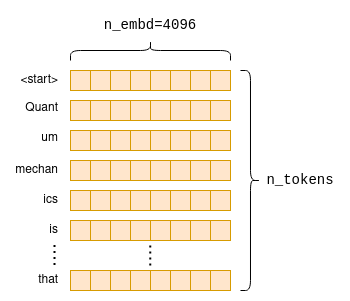
\includegraphics[width=0.5\linewidth]{llama_cpp_embedding.png}
        \caption[llama.cpp: Embedding matrix]{Details of the embedding matrix in llama.cpp~\cite{mallisUnderstandingHowLLM2023}. \lstinline|n_embd| is specific to the \gls{LLM}. The value depicted here is for Llama 2, a predecessor of Llama 3.2.}
        \label{fig:llamaCppEmbedding}
    \end{wide}
\end{figure}

With the prompt effectively converted into a matrix representation, the \gls{LLM} can now apply \textit{transformations} to it, i.e. multiply it with a series of matrices. \cref{fig:llamaCppTokenGeneration} depicts this as "Transformer layers with self-attention". This is the core of the \textit{Transformer} architecture introduced in 2017, which is the basis for most \glspl{LLM} today~\cite{vaswaniAttentionAllYou2023} (see \cref{sec:aShortHistoryOfLLMs} for some more details). Different variants of the Transformer architecture exist, namely encoder-decoder or decoder-only~\cite{mallisUnderstandingHowLLM2023}. They each come with their own strengths and weaknesses, the discussion of which is out of scope for this thesis. For us, it is only relevant that we want to support as many \glspl{LLM} as possible. This means we have to check if an encoding step is required before performing the decoding step. Fortunately, llama.cpp abstracts this away behind a simple function call each~\cite{gerganovGgerganovLlamacpp2024}. The result of these transformations is a matrix of logits, i.e. of unnormalized probabilities for the prediction of the next token~\cite{mallisUnderstandingHowLLM2023}. \cref{fig:llamaCppLogits} shows the logits matrix in detail. Its dimensions are \lstinline|n_tokens| $\times$ \lstinline|n_vocab|. \lstinline|n_vocab| is the vocabulary size specific to the \gls{LLM}, i.e. the number of tokens it knows~\cite{mallisUnderstandingHowLLM2023}.

\begin{figure}
    \begin{wide}
        \captionsetup{width=\linewidth}
        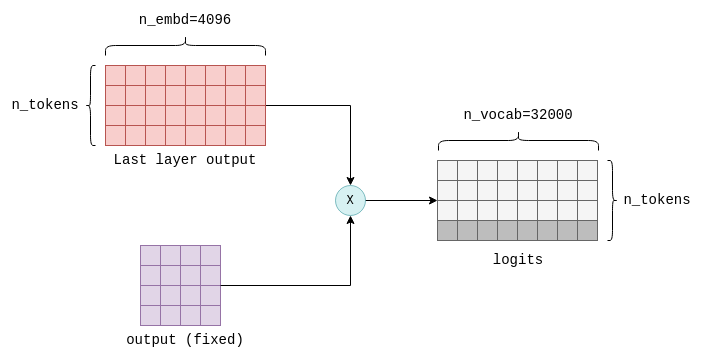
\includegraphics[width=\linewidth]{llama_cpp_logits.png}
        \caption[llama.cpp: Logit matrix]{Details of the logit matrix in llama.cpp~\cite{mallisUnderstandingHowLLM2023}. Also shown is the last transformation layer, i.e. the last intermediate matrix being multiplied with a fixed "output" matrix. This is not to be confused with the output of the \gls{LLM} as defined earlier.}
        \label{fig:llamaCppLogits}
    \end{wide}
\end{figure}

Each row of the logit matrix corresponds to a token in the prompt. It contains the logits (think: probabilities) for every token in the vocabulary to follow this token of the prompt. In other words, only the last row of the logit matrix is relevant for us, as it contains the logits for the last token of the prompt~\cite{mallisUnderstandingHowLLM2023}. This is highlighted in \cref{fig:llamaCppLogits}. Generally, these logits will be normalized to the interval $[0,1]$ using a softmax function (see \cref{sec:arithmeticCoding}). Only then they are interpretable as probabilities~\cite{mallisUnderstandingHowLLM2023,turnerIntroductionTransformers2024}.

Now we need to select the token to complete the prompt with based on the probabilities. This is called sampling~\cite{mallisUnderstandingHowLLM2023}. We will implement our own logic to encode information by sampling certain tokens, i.e. to encode the secret message when performing steganography (see \cref{sec:steganographyEncodingDecoding}). Furthermore, there are various different general-purpose sampling methods. The simplest is greedy sampling. Greedy sampling just selects the token with the highest probability to come next~\cite{mallisUnderstandingHowLLM2023}. This will be used in our implementation to finish the last sentence of the cover text when there is nothing of the secret message left to encode (see \cref{sec:finishingTheLastSentence}). Other common approaches are temperature sampling and top-k sampling~\cite{mallisUnderstandingHowLLM2023}. In temperature sampling, the probabilities are scaled with $1/temperature$ to modify their distribution. For $temperature < 1$ the distribution gets steeper around the most likely token, making the response more coherent. For $temperature > 1$ the distribution gets flatter, making the response less coherent ("more creative")~\cite{mallisUnderstandingHowLLM2023}. Top-k sampling only considers the tokens with the top k probabilities~\cite{mallisUnderstandingHowLLM2023}. Temperature sampling and top-k sampling will be combined when the \lstinline|Arithmetic| setting for steganography is chosen (see \cref{sec:settingsScreen,sec:arithmeticCoding} for details)~\cite{zieglerHarvardnlpNeuralSteganography2025}.

When a token is sampled, it is appended to the prompt to construct the response~\cite{mallisUnderstandingHowLLM2023}. The full response is built iteratively, so this output is used as input for the next iteration. This is also called autoregressive~\cite{mallisUnderstandingHowLLM2023}. Iteration stops when the \gls{LLM} samples a special end-of-generation token~\cite{gerganovGgerganovLlamacpp2024}. While the response in principle is ready now, it still is represented as a vector of token IDs. Before being displayed to the user as a string, it needs to be detokenized~\cite{mallisUnderstandingHowLLM2023}. The response after one iteration is shown in \cref{fig:llamaCppTokenGeneration}, after sampling the token "provides".

\section{Algorithms}
\label{sec:algorithms}

\subsection{Binary conversion and compression}
\label{sec:binaryConversionAndCompression}

\subsubsection{Arithmetic compression}
\label{sec:arithmeticCompression}

\subsubsection{Huffman compression}
\label{sec:huffmanCompression}

\subsubsection{UTF-8}
\label{sec:utf8}

\subsection{Steganography encoding/decoding}
\label{sec:steganographyEncodingDecoding}

\subsubsection{Arithmetic coding}
\label{sec:arithmeticCoding}

\subsubsection{Huffman coding}
\label{sec:huffmanCoding}

\section{Finishing the last sentence}
\label{sec:finishingTheLastSentence}
Our app is based on the Stegasuras project~\cite{zieglerNeuralLinguisticSteganography2019}. While we are able to use its algorithms for steganography, they come with an unsolved edge case. If cover text generation would stop as soon as the secret message is encoded, the last sentence would most likely be incomplete. Not finishing the last sentence is not an option, as it would make our communication highly suspicious to an attacker. A possible solution is performing greedy sampling until a suitable punctuation mark is reached. This is already demonstrated in Stegasuras~\cite{zieglerHarvardnlpNeuralSteganography2025}. But if we decode such a cover text, we get the secret message, followed by some noise. This is because the tokens from greedy sampling don't encode any actual information. Our app would provide a rather unpolished user experience if we left it like this.

We propose a solution to clean up this noise during decoding: A suitable stop signal is injected somewhere in the encoding process, appending it to the secret message. During decoding, we can thereby identify the end of the secret message. Any noise following the stop signal can then be cut off. The challenge is finding a step in the encoding process suitable for injection, which also determines the form of the stop signal.

We briefly recall how the secret message is encoded: First it gets converted from string to binary, compressing it in the process. Then it gets encoded into a cover text using the algorithm-specific sampling, followed by greedy sampling. It may also get encrypted between compression and cover text generation. Therefore, we cannot make any structural assumptions about the bit sequence being \textit{decoded} from the cover text. We have to insert our stop signal earlier in the encoding process, so that we can identify it later in the decoding process.

This ultimately led us to consider a special character as a stop signal. We append this special character to the secret message before it gets converted from string to binary. A suitable special character needs to be unlikely as organic user input, so that blocking it doesn't degrade the user experience significantly. The ASCII NUL character presents such a solution. While languages such as C and C++ use it for string termination, it doesn't serve any purpose in Kotlin. It doesn't have a visual representation either, and therefore is not on any standard keyboard. When appending it to the secret message, it introduces a small maximum overhead of 8 bits if UTF-8 is used for binary conversion. When the secret message is being compressed, the overhead is even less.

\section{Creating a conversation between cover texts}
\label{sec:creatingAConversationBetweenCoverTexts}
A \gls{LLM} fundamentally works by completing any prompt it is given (see \cref{sec:tokenGenerationWithLlamaCpp}). We are already able to leverage this for steganography by manipulating token generation, thereby encoding a secret message into a cover text (see \cref{sec:steganographyEncodingDecoding}). But we still don't have a way to create a conversation between cover texts. This means our first requirement (see \cref{ch:introduction}) is not fulfilled yet.

This section will show how creating a conversation between cover texts is possible. We will also show how to influence the \gls{LLM} behaviour on a lower level, via a system prompt. Both is achieved at once, by formatting the context as a conversation using special tokens~\cite{jiangChatBugCommonVulnerability2025}.

The context is formatted into a conversation by structuring it into messages. Each message has a role and a content~\cite{jiangChatBugCommonVulnerability2025}. There are three possible roles: System, user and assistant~\cite{jiangChatBugCommonVulnerability2025}. The system role is reserved for the system prompt. Its content is a natural language command the user can give the \gls{LLM} to influence its behaviour~\cite{jiangChatBugCommonVulnerability2025}. For the \gls{LLM}, the system prompt is always the first message of the conversation. In a typical \gls{UI} however, the system prompt is hidden away in the settings. Our implementation handles it like this too.

The user role is assigned to the subsequent prompts input by the user~\cite{jiangChatBugCommonVulnerability2025}. The assistant role is assigned to the responses output by the \gls{LLM}~\cite{jiangChatBugCommonVulnerability2025}. At the end of the formatted context, the special token for the assistant role is appended. This signals the \gls{LLM} to continue the conversation, i.e. to respond to the last message. Listing~\ref{lst:chatTemplate} shows an example.

% Add some space on top of listing to match bottom
\vspace{0.25cm}

\begin{lstlisting}[caption={[llama.cpp: Chat templates]{Example for a context formatted with the chat template of Llama 3.2 1B. Some line breaks have been added for readability.}}, label={lst:chatTemplate}]
<|start_header_id|>system<|end_header_id|>Let's do a role play. You and I are friends, texting with each other. We talk about what we did on the weekend. Be brief and casual, but friendly and engaging. Use emojis and phrases typical for chat messages.<|eot_id|>
<|start_header_id|>user<|end_header_id|>How was your weekend?<|eot_id|>
<|start_header_id|>assistant<|end_header_id|>
\end{lstlisting}

Unfortunately, the special tokens for context formatting are not uniform across \glspl{LLM}. Fortunately, llama.cpp has support for a wide range of formattings. In the vocabulary of llama.cpp, they are called chat templates~\cite{gerganovGgerganovLlamacpp2024,jiangChatBugCommonVulnerability2025}. We can query a \gls{LLM} for its chat template and pass this as a parameter to other functions. Thereby, we remain compliant with our fourth requirement of making the \gls{LLM} swappable (see \cref{ch:introduction}).

When completing the formatted context, the \gls{LLM} performs our algorithm-specific sampling (see \cref{sec:algorithms}). In doing so, we encode information in the next chat message and create a conversation from cover texts. Finally, our first requirement is fulfilled.

Strictly speaking, the conversation doesn't need to consist only of \textit{cover texts}. It may as well be composed of an arbitrary mixture of cover texts and plain texts, i.e. messages that don't encode a secret message. Our app allows this by letting the user toggle steganography on/off on the conversation screen (see \cref{sec:conversationScreen}). This gives the user great freedom to steer the topic of the conversation by sending plain text messages for non-sensitive communication. In addition to the system prompt, this enables us to improve cover text quality further.

Lastly, we mentioned that the \gls{LLM} needs to be able to talk \textit{to itself} (see \cref{sec:howToSelectASuitableLLM}). What we mean by this is that the \gls{LLM} is used by both chat partners to generate cover texts that are replies to the other chat partner. Consider this example: We have two chat partners, Alice and Bob. Alice wants to send a new cover text to Bob. The prior messages in the conversation are used as context. For encoding, Alice's prior messages have to be assigned the assistant role and Bob's prior messages have to be assigned the user role. When Bob receives this cover text, he has to replicate this state to decode it. When Bob wants to reply with another cover text, the roles are inversed. For encoding, Bob's prior messages have to be assigned the assistant role and Alice's prior messages have to be assigned the user role. Alice has to replicate this state to decode it. The roles are constantly switched following this pattern, effectively making the \gls{LLM} talk to itself without knowing it.

\section{Emojis}
\label{sec:emojis}
Emojis are widely used in instant messaging to express emotions, add visualizations or draw attention~\cite{zhouGoodbyeTextHello2017}. Being able to enrich our cover texts with this form of non-verbal communication is essential to make them seem organic. Today's \glspl{LLM} are able to output emojis when being prompted to (see \cref{sec:howToSelectASuitableLLM}). By demanding emojis in the system prompt, our app is able to do this as well. Accomplishing this however required some attention to detail. Therefore, we explain what needs to be considered when working with emojis and other non-ASCII characters in the context of the \gls{JNI} (see \cref{sec:jni}).

The \gls{JNI} is used to pass parameters between our Kotlin and C++ code. This requires conversions between the corresponding data types. For most data types this is simple, but for strings this is more sophisticated. This is due to collisions between different character encodings. As the ASCII encoding is contained in virtually all other encodings, pure ASCII strings generally are interoperable~\cite{gleaveMakingCompressionAlgorithms2017}. While the ASCII character set is sufficient for basic communication, it doesn't include emojis.

Emojis require the full Unicode character set. This can be encoded in various ways, the most common being UTF-8~\cite{gleaveMakingCompressionAlgorithms2017}. Consider the implementation of the \lstinline|LlamaCpp.detokenize| function in our source code: It detokenizes an array of token IDs back into a string using the \gls{JNI}. On the C++ side, one might be tempted call the \lstinline|NewStringUTF| function to create a \lstinline|jstring| object to pass back to Kotlin. While this works fine for ASCII strings, it makes our app crash when working with emojis. This is due to a \textit{modified} UTF-8 encoding being used by Java and therefore by the \gls{JNI}~\cite{oracleJNIFunctions}. To bypass this, we return the UTF-8 encoding of a string as a \lstinline|jbyteArray| instead. On the Kotlin side, we explicitly call the String constructor to specify that the bytes are UTF-8. This abstracts any Kotlin internals away.

While emojis now enable us to improve cover text quality, they introduce some further difficulties. When finishing the last sentence of the cover text during encoding, we use greedy sampling and terminate when reaching a suitable punctuation mark (see \cref{sec:finishingTheLastSentence}). To fulfill the third requirement defined in \cref{ch:introduction}, we have to keep cover texts as short as possible. If a cover text contains emojis, they may be used in place of punctuation marks to end a sentence~\cite{zhouGoodbyeTextHello2017}. But unlike punctuation marks, emojis cannot easily be detected using the Kotlin standard library. A simple approach like detecting non-ASCII characters would already conflict with the German letters ä, ö and ü, for example. A more sophisticated approach was implemented, using regular expressions to detect the Unicode categories containing emojis. But this didn't yield satisfying results as it corrupted a significant portion of cover texts. Therefore, cover texts including emojis only end when an appropriate punctuation mark is generated. This possibly makes them longer than necessary. But we consider it worth the trade-off, as the use of emojis can be easily influenced via the system prompt.
